\paragraph{1. Library toevoegen}
Om de navigatie en het laadscherm te kunnen gebruiken moeten we de juiste libraries aan 
de root van ons project toevoegen.
\begin{minted}{bash}
npm install @react-navigation/native
npm install react-native-screens
npm install react-native-safe-area-context
npm install @react-navigation/bottom-tabs
\end{minted}

\paragraph{2. onCreate methode toevoegen}
Om de navigatie te kunnen gebruiken moeten we een \textbf{onCreate} methode toevoegen aan het
\textit{android/app/src/main/java/com/project/MainActivity.java} bestand. Dit doen we door de 
volgende regels toe te voegen.
\begin{minted}{java}
import android.os.Bundle;
// ...
public class MainActivity extends ReactActivity {
  // ...
  @Override
  protected void onCreate(Bundle savedInstanceState) {
    super.onCreate(null);
  }
  // ...
}
\end{minted}

\paragraph{3. Dependencies toevoegen}
Om het laadscherm te kunnen gebruiken moeten we de juiste dependencies toevoegen aan het
\textit{android/app/build.gradle} bestand. Dit doen we door de volgende regels toe te voegen.
\begin{minted}{java}
dependencies {
  // Andere dependencies
  implementation("androidx.core:core-splashscreen:1.0.0")
}
\end{minted}

\paragraph{4. Laadscherm toevoegen}
Eerst genereren we een Laadscherm met behulp van een commando aangeboden door de library.
\begin{minted}{bash}
npx react-native generate-bootsplash path/to/icon.png
    --background-color "#000000" 
    --logo-width=100 
    --assets-path=assets 
    --flavor=main 
    --platforms=android,ios
\end{minted}
Daarna maken we een stijl om het laadschem te tonen. Dit doen we door de volgende regels toe te
voegen aan het \textit{android/app/src/main/res/values/styles.xml} bestand.
\begin{minted}{xml}
<style name="BootTheme" parent="Theme.SplashScreen">
    <item name="windowSplashScreenBackground">@color/bootsplash_background</item>
    <item name="windowSplashScreenAnimatedIcon">@mipmap/bootsplash_logo</item>
    <item name="postSplashScreenTheme">@style/AppTheme</item>
</style>
\end{minted}
Om het laadscherm dan als eerste te tonen moeten we de volgende regels toevoegen aan het
\textit{android/app/src/main/AndroidManifest.xml} bestand.
\begin{minted}{xml}
<application
  android:name=".MainApplication"
  android:label="@string/app_name"
  android:icon="@mipmap/ic_launcher"
  android:roundIcon="@mipmap/ic_launcher_round"
  android:allowBackup="false"
  android:theme="@style/BootTheme"> <!-- Verander deze lijn -->
  <!-- ... -->
</application>
\end{minted}
Tot slot initialiseren we het laadscherm door de volgende regels toe te voegen aan het
\textit{android/app/src/main/java/com/project/MainApplication.java} bestand.
\begin{minted}{java}
import com.zoontek.rnbootsplash.RNBootSplash;

public class MainApplication extends Application implements ReactApplication {
  // ...
  @Override
  public void onCreate(Bundle savedInstanceState) {
    RNBootSplash.init(this); // Voeg deze lijn toe
    super.onCreate(savedInstanceState);
  }
  // ...
}
\end{minted}

\paragraph{5. Navigatie toevoegen}
Om de navigatie te kunnen gebruiken moeten we alle alle componenten in een 
\textbf{NavigationContainer} component steken. Dit doen we door de volgende regels toe te voegen
aan het \textit{App.tsx} bestand.
\begin{minted}{typescript}
import { NavigationContainer } from '@react-navigation/native';

export default function App() {
  return (
    <NavigationContainer>
      {/* ... */}
    </NavigationContainer>
  );
}
\end{minted}

\paragraph{6. Bottom Tab navigatie toevoegen}
Om de bottom tab navigatie te kunnen gebruiken moeten we een \textbf{createBottomTabNavigator}
functie aanmaken. Dit doen we door de volgende regels toe te voegen aan het \textit{App.tsx} bestand.
\begin{minted}{typescript}
import { createBottomTabNavigator } from '@react-navigation/bottom-tabs';

const Tab = createBottomTabNavigator();

export default function App() {
  return (
    <NavigationContainer>
      <Tab.Navigator>
        {/* ... */}
      </Tab.Navigator>
    </NavigationContainer>
  );
}
\end{minted}
Daarna kunnen we nog de verschillende schermen toevoegen aan de \textbf{Tab.Navigator} component.
\begin{minted}{typescript}
<Tab.Navigator>
    <Tab.Screen name="Home" component={HomeScreen} />
    <Tab.Screen name="Second" component={SecondScreen} />
    <Tab.Screen name="Third" component={ThirdScreen} />
</Tab.Navigator>
\end{minted}

\paragraph{7. Applicatie maken}
Met deze informatie maken we een applicatie met een laadscherm dat zal verdwijnen vanaf de 
applicatie gerenderd is. Daarna is er een bottom tab navigatie dat navigeert tussen 
de drie verschillende schermen. 
\begin{figure}[H]
    \centering
    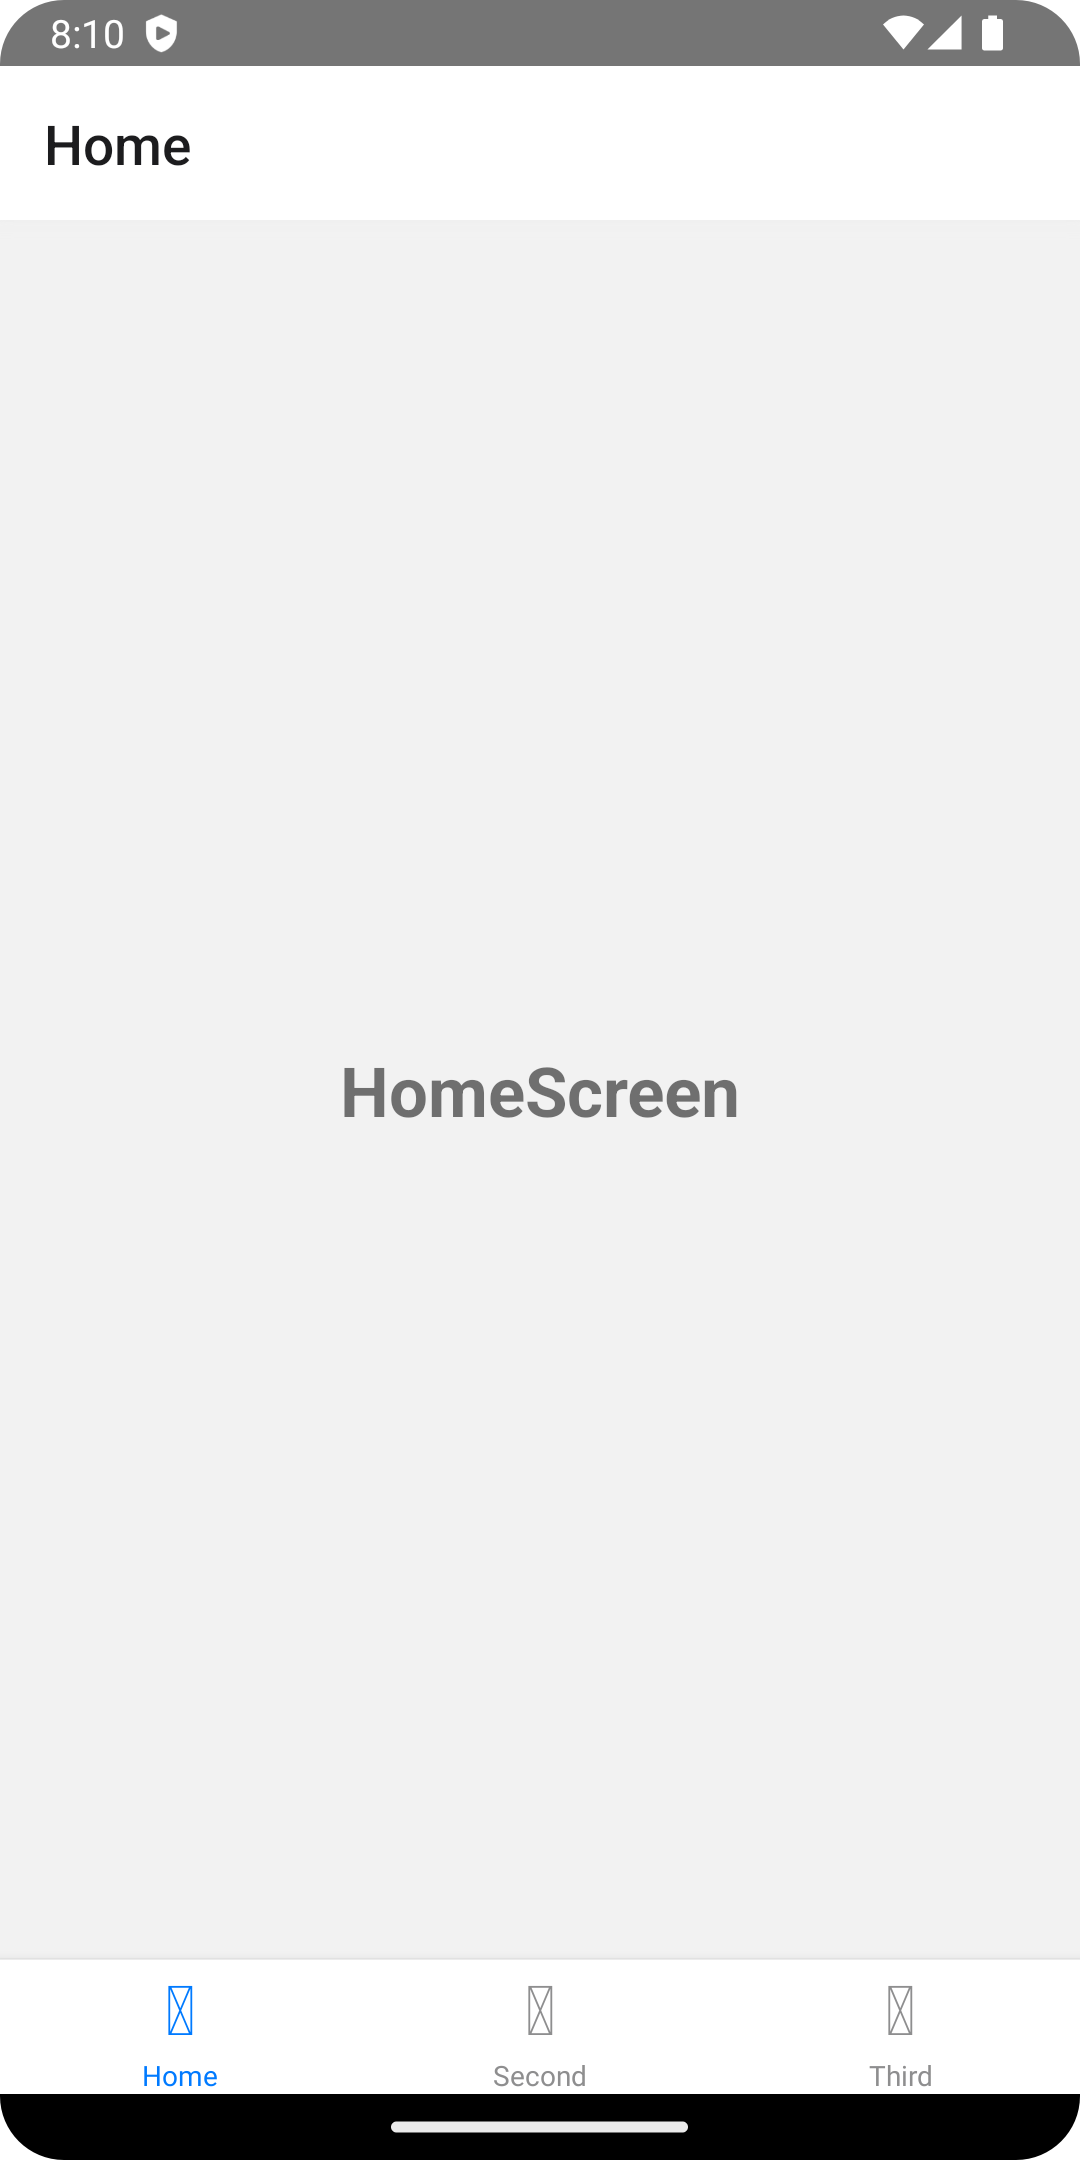
\includegraphics[height=0.4\textheight]{basis_layoutcross.png}
    \caption{Layout van applicatie voor de basisfunctionaliteiten bij React Native.}
\end{figure}